\documentclass[12pt,journal,compsoc]{IEEEtran}
\usepackage[english]{babel}
\usepackage[utf8]{inputenc}
\usepackage[left=2cm,right=2cm,top=1cm,bottom=2cm]{geometry}

\usepackage{amssymb}
\usepackage{amsmath}
\usepackage{array}
\usepackage{biblatex}
\usepackage{blindtext}
\usepackage{booktabs}
\usepackage{caption}
\usepackage{csquotes}
\usepackage{fancyhdr}
\usepackage{hyperref} 
\usepackage{listings}
\usepackage{url}
\usepackage{verbatim}
\usepackage{xcolor}

\usepackage[dvipdfmx]{graphicx}

\geometry{a4paper, margin=1in}

\renewcommand{\thefigure}{\arabic{figure}.0}

\bibliography{References}

% Define custom colors
\definecolor{codegreen}{rgb}{0,0.6,0}
\definecolor{codegray}{rgb}{0.5,0.5,0.5}
\definecolor{codepurple}{rgb}{0.58,0,0.82}
\definecolor{backcolour}{rgb}{0.95,0.95,0.92}

\hypersetup{
    colorlinks=true,
    linkcolor=blue,
    filecolor=magenta,      
    urlcolor=cyan,
    pdftitle={AIEA Report},
    pdfpagemode=FullScreen,
}
\urlstyle{same}

% Indent setting
\setlength{\parindent}{0pt}

% Define custom style for listings
\lstdefinestyle{mystyle}{
    backgroundcolor=\color{backcolour},   
    commentstyle=\color{codegreen},
    keywordstyle=\color{magenta},
    numberstyle=\tiny\color{codegray},
    stringstyle=\color{codepurple},
    basicstyle=\ttfamily\footnotesize,
    breakatwhitespace=false,         
    breaklines=true,                 
    captionpos=b,                    
    keepspaces=true,                 
    numbers=left,                    
    numbersep=5pt,                  
    showspaces=false,                
    showstringspaces=false,
    showtabs=false,                  
    tabsize=2
}

% Apply the custom style to all listings
\lstset{style=mystyle}

\usepackage{epstopdf}
\usepackage{graphicx}
\usepackage{url}
\usepackage{hyperref}
\usepackage[T1]{fontenc}
\usepackage{amsmath,amssymb}
\usepackage{mhchem}
\usepackage{pgfplots}

%###########################
% Header
%###########################

\begin{document}
\title{Title}
\author{YourName\\
        \small{Here is BIOGRAPHY}}
\date{}

\IEEEtitleabstractindextext{
\begin{abstract}
  Here is abstract
\end{abstract}}
  
\maketitle

%###########################
% Page
%###########################
\markboth{IEEE}
\IEEEpubid{YourName}

\section{Introduction}

\IEEEPARstart{W}{elcome}

\subsection{Subsection}

Here is the list element. 
\begin{enumerate}
  \item Here is the list element.  
  \item Here is the list element. 
  \item Here is the list element.  
  \item Here is the list element. 
\end{enumerate}

\subsection{Example: Two Columns, Three Rows}
\begin{table}[h]
  \renewcommand{\arraystretch}{1.2}
  \caption{Sample Table (2 Columns, 3 Rows)}
  \label{table:sample}
  \centering
  \begin{tabular}{|c|c|}
  \hline
  \textbf{Column 1} & \textbf{Column 2}\\
  \hline
  Row 1 & Data 1\\
  \hline
  Row 2 & Data 2\\
  \hline
  Row 3 & Data 3\\
  \hline
  \end{tabular}
\end{table}

\section{Figures}

\begin{figure}[h!]
  \centering
  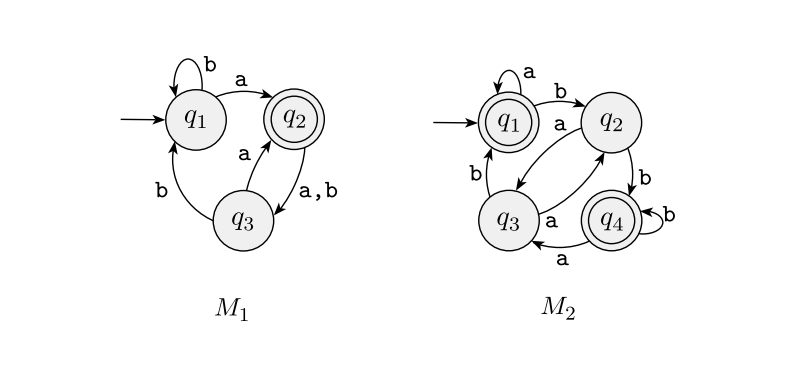
\includegraphics[width=\linewidth, height=10.0em, keepaspectratio]{./img/p1.1.png}
  \caption{Graph on Question 1.4-g}
  \label{fig:DFStopo}
\end{figure}

\subsection{Plotting the Data}
Below is an example of embedding data directly in a \verb|tikzpicture| environment:

\begin{figure}[h]
    \centering
    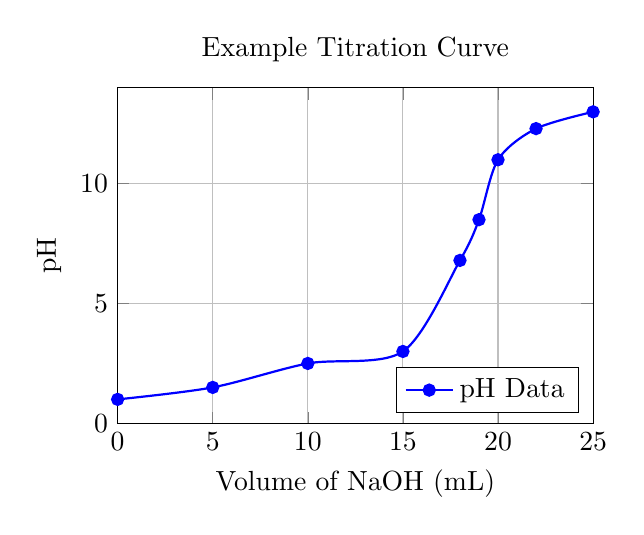
\begin{tikzpicture}
        \begin{axis}[
            width=3in,
            height=2.3in,
            grid=major,
            xlabel={Volume of NaOH (mL)},
            ylabel={pH},
            xmin=0, xmax=25,
            ymin=0, ymax=14,
            title={Example Titration Curve},
            legend pos=south east
        ]
        \addplot[
            smooth,
            thick,
            mark=*,
            color=blue,
            table/x index=0,
            table/y index=1
        ] table {
            0   1.0
            5   1.5
            10  2.5
            15  3.0
            18  6.8
            19  8.5
            20  11.0
            22  12.3
            25  13.0
        };
        \legend{pH Data}
        \end{axis}
    \end{tikzpicture}
    \caption{Plot of example pH data versus volume of \ce{NaOH} added.}
    \label{fig:titrationPlot}
\end{figure}

\end{document}